\section{Introduction}
A long-term goal of robotics research is the introduction of
intelligent household robots.  To be effective, such robots will need
to perform complex tasks over long horizons (e.g., setting a dinner
table, doing laundry). Planning for these long-horizon tasks is
infeasible for state-of-the-art motion planners, making the need for a
hierarchical system of reasoning apparent.

One way to approach hierarchical planning is through combined
\emph{task and motion planning} (TAMP). In this approach, an agent is
given a symbolic, logical characterization of actions (e.g., move,
grasp, putdown), along with a geometric encoding of the
environment. TAMP systems maintain a hierarchical separation of
high-level, symbolic task planning and low-level, geometric motion
planning.  Efficient integration of these two types of reasoning is
difficult, and recent research has proposed several methods for
it~\cite{srivastava2014combined, deardenplanningtamp, kaelbling2011hierarchical,
  lagriffoul2014orientation, GarrettWAFR14, dornhege2012semantic}.
We adopt the principles of abstraction in the TAMP system developed by
Srivastava et al.~\cite{srivastava2014combined} (henceforth referred
to as SFRCRA-14) to factor the reasoning and search problems into
interacting logic-based and geometric components.

\begin{figure}[t]
  \centering
    \noindent
    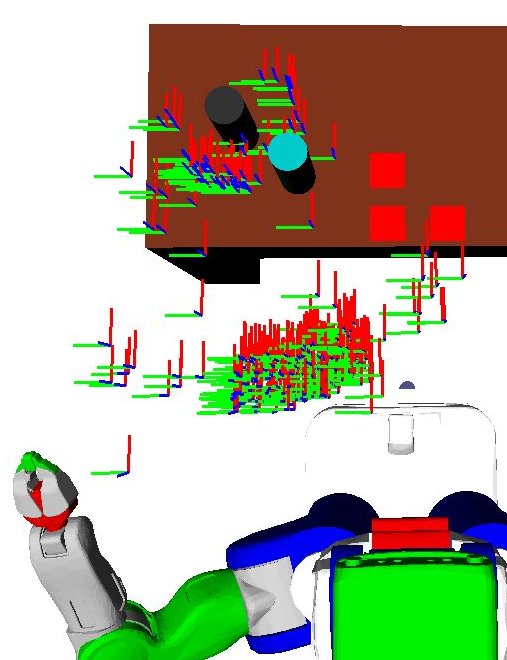
\includegraphics[scale=0.15]{images/move_grasp.png}\hspace{6 mm}
    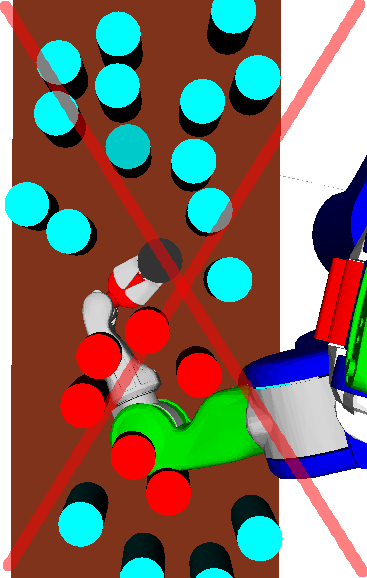
\includegraphics[scale=0.19]{images/grasp_teaser_bad.png}
    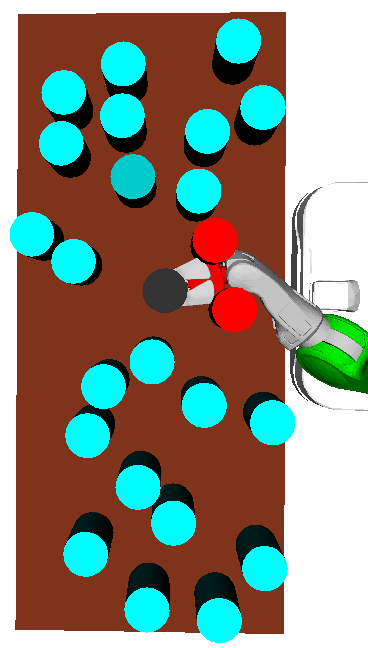
\includegraphics[scale=0.185]{images/grasp_teaser_good.png}
  \caption{\small{\textbf{Left}: We use reinforcement learning to train good sampling distributions for
      continuous motion planning parameters in long-horizon tasks.
      The image shows learned base position (blue) and
      grasping (green) distributions for picking up the black can. The grasping
      policy learned to avoid the obstructions. The green points refer
      to the position of the tool center point; the end effector is oriented
      to point toward the object being grasped. \textbf{Right}: When trying to grasp the black can, the sampled grasping pose can
      significantly affect the quality of the obstructions determined. The new plan proposed from the rightmost image only
      requires moving 2 obstructions out of the way, versus 6 from the other. We integrate inverse reinforcement learning into our task and
      motion planning system to learn an ordering on plan exploration, causing the system to prefer simpler and more feasible plans.}}
  \label{fig:cover}
\end{figure}

In this work, we develop a complete algorithm for TAMP and propose
methods for jointly carrying out guided search in the space of
high-level (logic-based) plans and their low-level
\emph{refinements}: instantiations of continuous values for
symbolic references in the plan. We refer to this search for a valid low-level
refinement as \emph{plan refinement}.

Our complete algorithm introduces
a \emph{plan refinement graph}, a data structure that stores a
set of qualitatively different high-level plans that could solve a task.
During planning, we repeatedly select one such plan and either try to
refine it or incorporate geometric information to generate a new high-level
plan. This allows interleaving plan refinement with a
search over \emph{which} high-level plan to try refining, given options
that address different infeasibilities.

We present machine learning techniques to train heuristic functions that guide
both of these search processes. At the high level, this amounts to learning
to predict how difficult it is to refine a given plan. We use inverse reinforcement learning
based on expert demonstrations to estimate this quantitatively, using a max-margin formulation.
At the low level, training heuristics amounts to
learning to propose continuous values (for symbolic references) that are likely to result in
collision-free trajectories. Many TAMP systems rely on hand-coded heuristics to
account for these continuous parameter settings. This often requires
domain-specific insight from the user to reduce the search space.
We apply reinforcement learning (RL) to learn domain-specific distributions
over these values in a domain-independent fashion.

Our learning approach draws inspiration
from Zhang and Dietterich~\cite{JobShopSched}, who applied RL to job
shop scheduling. In their formulation, states correspond to schedules
and actions propose changes to the schedule. In our setting, states
correspond to (potentially infeasible) refinements and actions propose
new values for symbolic references.

The contributions of our work are as follows: 1) we present a complete
algorithm for TAMP by maintaining a plan refinement graph; 2) we
present a local search algorithm for plan refinement that is easily
formulated as an MDP; 3) we formulate plan refinement in the RL
framework and learn a policy for this MDP; 4) we use inverse RL with
expert demonstrations to train heuristics for
searching intelligently through a plan refinement graph; and 5) we
present experiments to evaluate our approach in a variety of simulated
domains. Our results demonstrate that our approach yields
significantly improved performance over SFRCRA-14.
